\section{Protein Extraction and Analysis\authorB{}}
\subsection{Protein Extraction}
To control the binding of REEs, lanmodulin has to be extracted from bacteria cells.
This is done with the following steps:

\textbf{Lysis: Breaking the Cellular Wall}

As already discussed in~\ref{sec:me_lysis} lysis involves breaking open the bacterial cells to access the intracellular proteins.
This is achieved through our chosen methods:

\begin{itemize}
    \item \textbf{Shock frosting:} \\
    \begin{figure}[H]
                  \centering
                  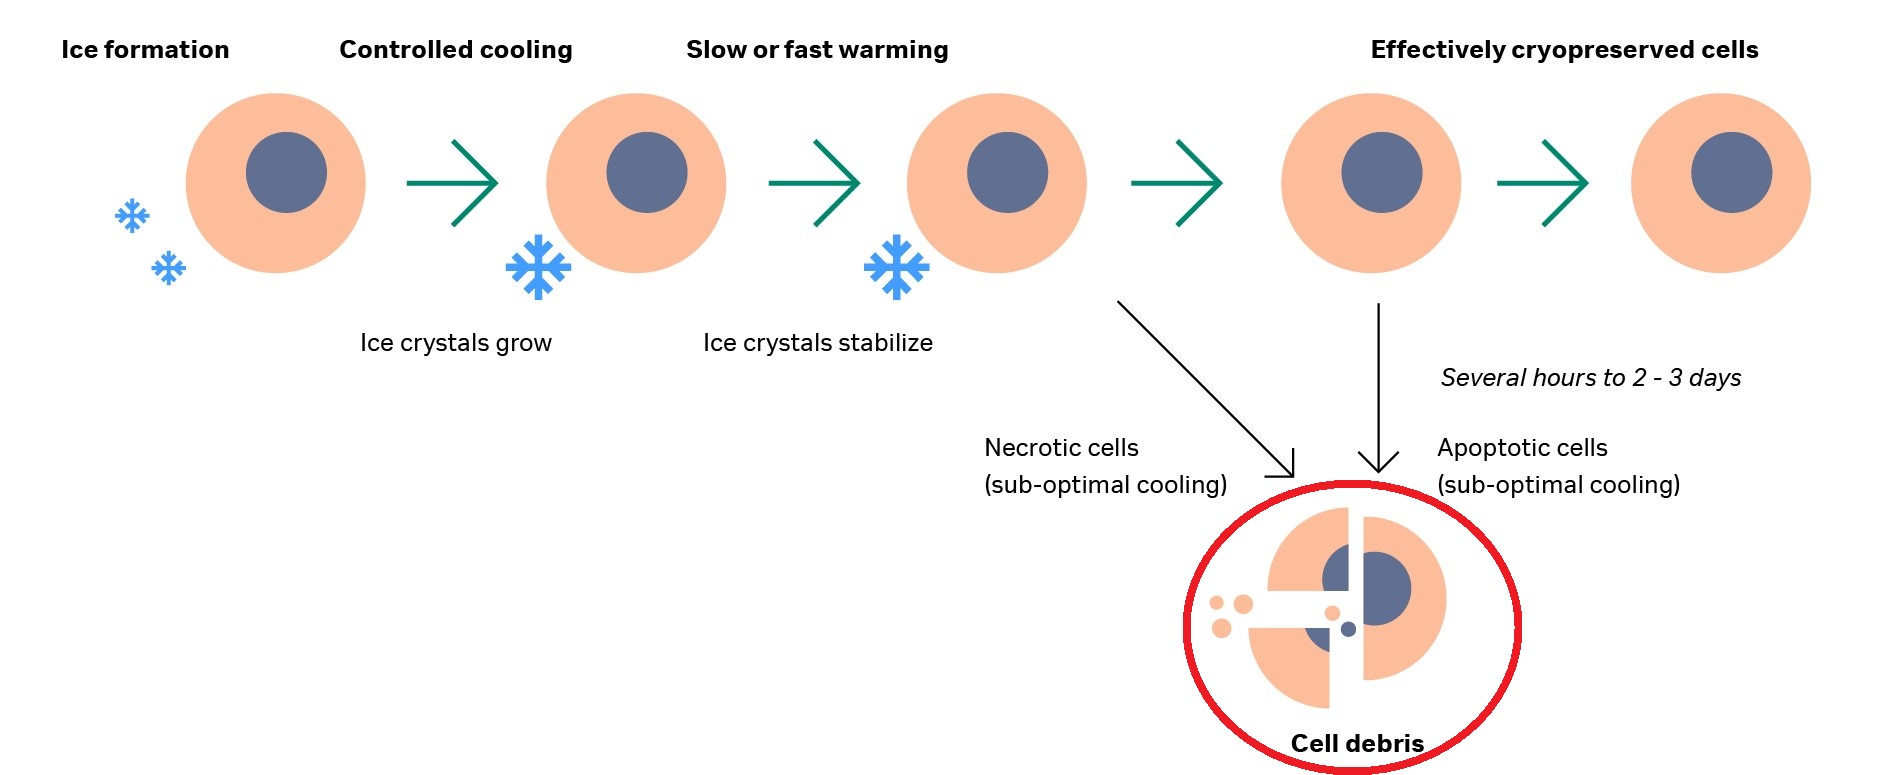
\includegraphics[width=1\textwidth]{./media/images/shock_frosting_cell}
                  \caption{Lysis is induced after what is described as "suboptimal cooling", which in our case is the wanted outcome (red circle). Picture from Cytiva, with modifications.}
                  \label{fig:shock_frosting_cell}
    \end{figure}
    Shock frosting, also known as freeze-thaw lysis, is a physical method used to disrupt
    bacterial cells by subjecting them to rapid temperature changes.
    The process involves freezing the bacterial culture rapidly at low temperatures like -80°C in our case, followed by thawing them at medium temperatures about 38°C to not coagulate the protein.
    The rapid freezing causes the formation of ice crystals, which physically
    disrupt the cell membrane.
    Upon thawing, the ice crystals melt, leading to further
    mechanical stress on the cellular structures, eventually resulting in cell lysis and the release of intracellular components. \\
    In the case of \emph{Methylorubrum extorquens}, shock frosting was an effective way to
    disrupt cellular integrity, releasing intracellular proteins like lanmodulin.

    \newpage
    \item \textbf{Sonication:} \\
    \begin{figure}[H]
        \centering
        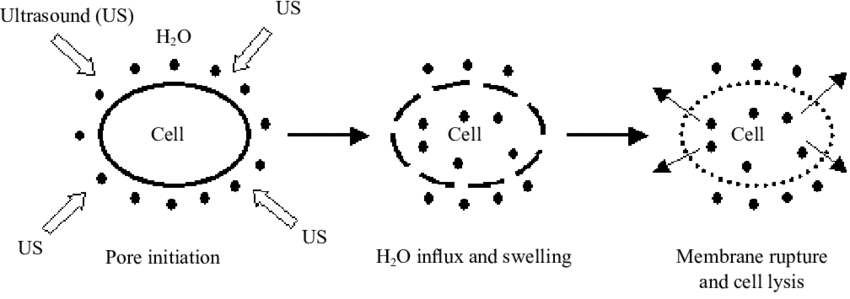
\includegraphics[width=1\textwidth]{./media/images/ultrasound_cell}
        \caption{Schematic of cell rupture with ultrasound. Picture from "Ultrasound in Process Engineering", Nikitenko and Chemat~\cite{ultrasoundcell}.}
        \label{fig:ultrasound_cell}
    \end{figure}
    Sonication, or ultrasonication, is a mechanical method used to disrupt bacterial cell
    walls through the application of high-frequency sound waves.
    In this method, the bacterial culture is subjected to ultrasonic waves generated by a sonicator probe or bath.
    The high-frequency waves create alternating cycles of compression and rarefaction within the culture medium, generating cavitation bubbles.
    These bubbles undergo rapid expansion and collapse, generating intense shear forces and
    microstreaming, which disrupt the cell membrane and cell wall. \\
    Sonication is particularly effective for lysing tough bacterial cell walls, including those of gram-negative bacteria like \emph{Methylorubrum extorquens}.
    However, it is essential to optimize sonication parameters such as amplitude, duration, and temperature to avoid excessive heating and denaturation of sensitive intracellular components.
    Sonication was the final step for effective lysis and disruption of \emph{M. extorquens} cell walls.
\end{itemize}

\textbf{Cell Debris Removal}

After cell disruption, the lysate (cell extract) contains a mixture of cellular components,
including proteins, membranes, and nucleic acids.
To isolate the proteins, unwanted components were removed by centrifugation.
The lysate is spun at high speeds in a centrifuge.
This separates the heavier cell debris (pellet) from the soluble components
(supernatant) containing the proteins.

Throughout this process, protein concentration and purity were monitored using techniques
like SDS-PAGE and IR-Spectrometry respectively, more on these methods and their
effectiveness later.
To keep the amino acids intact, the epi containing the bacteria needed to be cooled all the time.
This prevented protease from consuming and therefore destroying the amino acids of our interest.

\newpage

\subsection{IR-Spectroscopy}
Infrared (IR) spectroscopy has established itself as a cornerstone analytical technique across diverse scientific fields.
Its ability to elucidate the structural characteristics of molecules stems from the fundamental interaction between atoms and infrared radiation, providing invaluable insights into the presence of functional groups and the unique vibrational fingerprint of each molecule.

\textbf{Theory:}

The theoretical foundation of IR spectroscopy is based on the well-established principle that molecules can undergo vibrational motion when exposed to specific frequencies of infrared radiation, the radiation matching the molecule's frequency is absorbed.
This radiation occupies a distinct region within the electromagnetic spectrum, encompassing wavelengths ranging from approximately 2.5 µm to 16 µm.
Unlike ultraviolet-visible (UV-Vis) spectroscopy, which excites electrons to higher energy levels, the energy associated with infrared radiation is insufficient for electronic transitions.
Instead, it triggers vibrations within the covalent bonds of the molecule.

The concept of vibrational modes is important to understanding IR spectroscopy.
These modes represent the various ways in which the atoms within a molecule can vibrate relative to each other.
These atoms are connected by bonds.
Stronger bonds, characterized by higher bond energies, vibrate at higher frequencies, while weaker bonds exhibit lower vibrational frequencies.
This distinctive correlation between bond type and vibrational frequency forms the cornerstone of IR spectroscopy.

\begin{figure}[H]
    \centering
    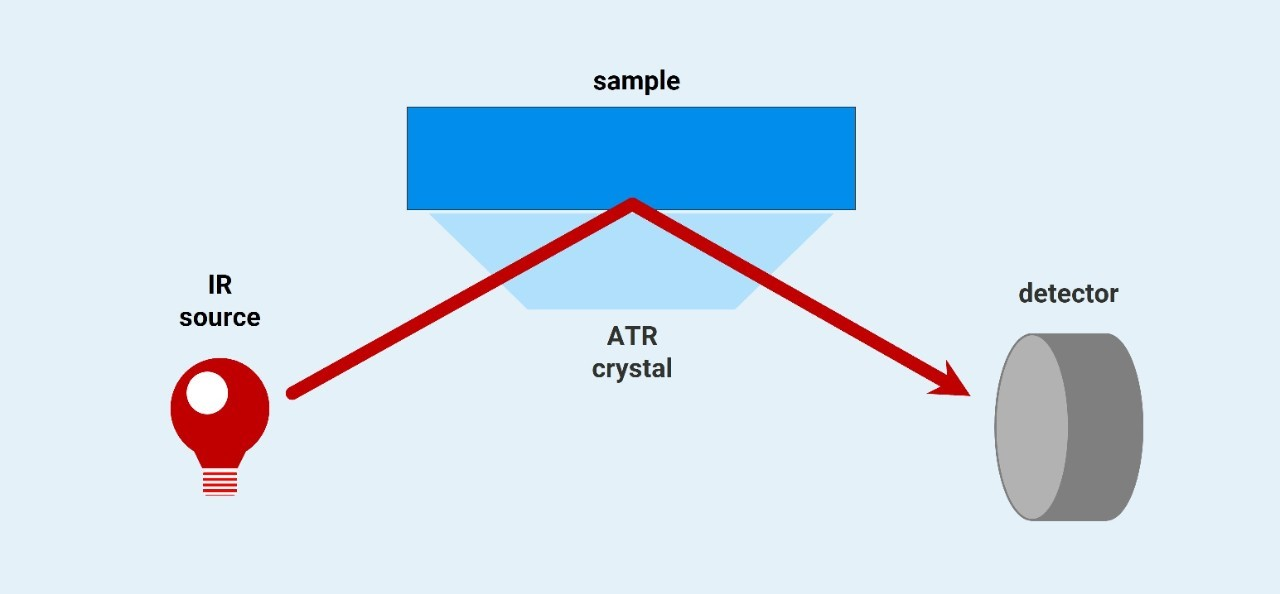
\includegraphics[width=0.9\textwidth]{./media/images/ir_spectrometer}
    \caption{Schematic of the reflection of IR light in an ATR (Attenuated Total Reflectance) Spectrometer.}
    \label{fig:ir_spectrometer}
\end{figure}

\textbf{The Infrared Spectrometer}

This instrument houses a light source that emits a broad spectrum of infrared radiation.
The prepared sample, in either solid, liquid, or gas phase, is positioned within the path of this radiation.
As the infrared light traverses the sample, specific frequencies corresponding to the molecule's vibrational modes are absorbed.
The remaining radiation is subsequently reflected and detected, and a spectrum is generated.
This spectrum typically presents the intensity of transmitted or absorbed light (y-axis) versus the frequency or wavelength (x-axis).

\textbf{Modes:}

Transmission Mode: In this mode, the infrared radiation directly transmits through the sample.
The resulting spectrum depicts the frequencies absorbed by the molecule, and it is the most commonly employed mode for solid and liquid samples.

Reflection Mode: This mode finds particular utility when analyzing samples that are challenging to prepare as thin films for transmission measurements.
In this case, the infrared radiation is directed onto the sample's surface, and the reflected light is captured.
The spectrum reflects the molecule's vibrational modes based on the analysis of the reflected frequencies.
For the analysis of \emph{Methylorubrum extorquens}, this mode was chosen simply because of the available equipment.

\textbf{Deciphering the Spectrum:}

The IR spectrum generated from the experiment bears a resemblance to a unique fingerprint for each molecule.
The x-axis typically displays the wavelength.
The y-axis represents the intensity of the absorption (or transmittance).
The spectrum usually shows diverse peaks,each corresponding to a specific vibrational mode within the molecule.
The location of a peak indicates the type of bond vibration that occurred, while the peak's intensity reflects the strength of the absorption.

By drawing upon extensive reference databases and theoretical calculations, the IR spectrum
can be interpreted to glean valuable information about the sample.
The presence of specific peaks can confirm the existence of particular functional groups, such as carbonyls (\ce{C=O}), alkenes (\ce{C=C}), and alcohols (\ce{O-H}).
The relative intensities of these peaks can even provide insights into the molecule's environment and interactions with neighboring molecules.

\newpage

\subsection{SDS-PAGE\authorB}
Outlining the key aspects of SDS-PAGE, a powerful method of protein analysis.
Proteins can be separated by size through a process called electrophoresis.
This involves applying an electric field to a polyacrylamide gel, which acts as a molecular sieve.
The proteins are then forced through the gel based on their size, with smaller proteins moving through faster than larger ones.

\subsubsection{Principles of SDS-PAGE}

\textbf{Protein Denaturation and Linearization with SDS}

Proteins are biomolecules with three-dimensional structures influenced by various interactions, including hydrogen bonds, disulfide bridges, hydrophobic interactions, and ionic bonds.
These interactions dictate a protein's function and overall shape.
However, for separation by size in SDS-PAGE, protein conformation becomes irrelevant.
This is achieved by sodium dodecyl sulfate (SDS), a strong anionic detergent.

SDS disrupts the noncovalent interactions within proteins, leading to their denaturation.
This process unfolds the protein and disrupts its native conformation. Importantly, SDS
binds to the unfolded polypeptide chain in a 1:1 ratio along its entire length~\cite{sdspageassay}. This
binding is primarily driven by hydrophobic interactions between the hydrocarbon tail of
SDS and the hydrophobic amino acid side chains within the protein~\cite{sdsimpact}.

A crucial consequence of SDS binding is the masking of a protein's inherent charge. Since
proteins possess a diverse array of amino acid side chains with varying pKa values, their
net charge at a specific pH can be positive, negative, or neutral. However, with SDS bound
along the entire polypeptide chain, the negatively charged sulfate groups of SDS
dominate the protein's overall charge. This imparts a negative charge proportional to the
protein's mass (due to the constant 1:1 SDS-to-protein ratio).

\begin{figure}[H]
    \centering
    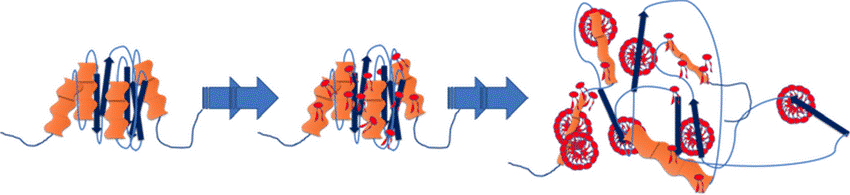
\includegraphics[width=0.8\textwidth]{./media/images/sds_effect}
    \caption{Representation of the denaturation effect of a protein promoted by SDS.}
    \label{fig:sds_effect}
\end{figure}

\subsubsection{Polyacrylamide Gels and Molecular Sieving}

The separation of proteins in SDS-PAGE is achieved through electrophoresis, a technique
that utilizes voltage to move charged molecules through a gel matrix. In SDS-PAGE, the
gel matrix is typically composed of polyacrylamide. This synthetic polymer forms a crosslinked network with pores of varying sizes. The pore size distribution within the gel is
determined by the percentage of acrylamide used during gel preparation~\cite{sdsgelsieving}.

During electrophoresis, the negatively charged SDS-protein complexes migrate towards
the positive electrode (anode) within the applied voltage. However, their movement is
impeded by the polyacrylamide gel matrix. Smaller proteins with minimal hindrance by
the gel pores navigate through the network more efficiently, resulting in faster migration.
Conversely, larger proteins encounter greater resistance within the tighter pores, leading
to slower migration.

This is known as molecular sieving and forms the basis of protein separation by size in
SDS-PAGE. Proteins are effectively ``sieved'' through the gel matrix, with smaller proteins
traveling further compared to larger ones. Ultimately, the distance migrated by each
protein in the gel reflects its molecular weight, allowing for the creation of a protein
profile based on size.

\begin{figure}[H]
    \centering
    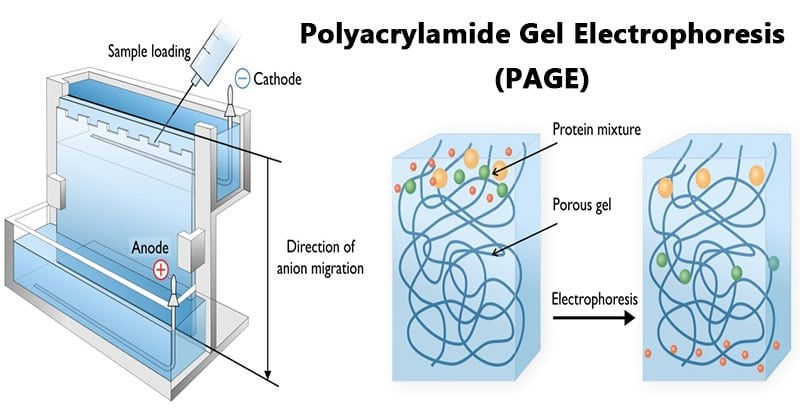
\includegraphics[width=0.8\textwidth]{./media/images/sds_schematic}
    \caption{SDS-PAGE schematic, (left) SDS-PAGE apparatus, (right) schematic of protein passing through porous gel.}
    \label{fig:sds_schematic}
\end{figure}

\subsubsection{Additional Considerations}
While SDS-PAGE is a powerful technique, a few points require consideration:

Disulfide Bridges: SDS does not disrupt disulfide linkages between cysteine residues.
Proteins with multiple disulfide bridges may have reduced mobility compared to their
predicted molecular weight based on linear sequence.

Glycosylation: The presence of sugar moieties (glycosylation) can slightly affect protein
mobility due to increased size and potential interactions with the gel matrix.
Protein-SDS Interactions: In rare cases, specific protein-SDS interactions may alter the
expected migration pattern.

Acrylamide: Usage of Acrylamide requires careful deployment and adequate protection
measures. Acrylamide is a toxic neurotoxin that poses a serious health risk when brought
in contact with skin, especially mucous membranes.

Curing issues: When implemented into research regarding Lanmodulin and REE recycling,
the issue of premature hardening or no hardening occurred. It is not yet clear why the
consistency of the gel changed too fast or slow when repeated multiple times with the
same amount of chemicals used.

Despite these limitations, SDS-PAGE remains a cornerstone technique in protein analysis
due to its simplicity, and reproducibility.

\newpage